\documentclass[conference]{IEEEtran}

\usepackage[T1]{fontenc}
\usepackage[table]{xcolor}
\usepackage{graphicx}
\usepackage{booktabs}
\usepackage{amsmath,amssymb}
\usepackage{tikz}
\usetikzlibrary{arrows.meta,positioning,shapes.geometric}
\usepackage{listings}
\usepackage{url}
\usepackage{cite}
\usepackage{hyperref}
\usepackage{balance}

\definecolor{docintelNavy}{HTML}{173B63}
\definecolor{docintelBlue}{HTML}{2F75B5}
\definecolor{docintelLightBlue}{HTML}{DCEBFA}
\definecolor{docintelPaleBlue}{HTML}{F1F7FC}
\hypersetup{colorlinks=true,linkcolor=docintelNavy,citecolor=docintelNavy,urlcolor=docintelBlue}
\definecolor{codegray}{gray}{0.95}
\lstset{basicstyle=\ttfamily\footnotesize,backgroundcolor=\color{docintelPaleBlue},rulecolor=\color{docintelBlue},
        breaklines=true,frame=single,captionpos=b,columns=fullflexible}

\title{DocIntel: A Provider-Flexible, Privacy-Oriented Document Intelligence Workspace\\
\large System Design, Implementation, and Evaluation}

\author{
\IEEEauthorblockN{Samar Mittal\hspace{1.5em}Rajkumar Santra\hspace{1.5em}Sonam Maurya}
}
\begin{document}
\maketitle
\vspace{-0.75em}

\begin{abstract}
Modern document repositories contain heterogeneous content, including text-native files, scanned pages, spreadsheets, tables, URLs, and multimedia sources. This paper presents DocIntel, a containerized document-intelligence workspace that combines document extraction, optional layout-aware optical character recognition (OCR), vector retrieval, provider-selectable generative models, notebook-oriented conversation, and downloadable visual explanations. The system separates the browser interface, API, processing workers, model providers, and persistent storage, while supporting local and cloud AI providers. The implementation uses Next.js, FastAPI, LangGraph/LangChain orchestration, SurrealDB, and optional Docling processing. This paper documents the architecture, retrieval workflow, privacy boundaries, implementation methodology, reproducibility procedure, and source-grounded evaluation of the system. Extraction succeeded for all 14 documents in the evaluated railway corpus. In a fixed 10-question benchmark, DocIntel answered all 10 questions correctly with Gemini 3.5 Flash Lite. Direct OpenCode/OpenRouter comparisons showed that Thinking Machines Inkling Small answered 10/10 correctly, while Cohere North Mini answered 8/8 usable questions correctly but produced provider failures for two invocations; GLM, Nemotron Lightning, and Nemotron Super VL produced usable text for only two questions in the reported run. Provider/process failures are therefore reported separately from semantic correctness. OCR, vision, retrieval ranking, and statistical robustness remain important future evaluations rather than claims established by this text-only benchmark.
\end{abstract}

\begin{IEEEkeywords}
Document intelligence, retrieval-augmented generation, OCR, vector search, knowledge workspace, multilingual interfaces, document layout analysis, provider interoperability
\end{IEEEkeywords}

\section{Introduction}
Organizations and researchers increasingly work with large, heterogeneous collections of documents. Conventional repositories support storage and keyword search but provide limited support for source-grounded question answering, cross-document synthesis, visual reasoning, or structured transformation. Information can also be lost when a document contains scans, complex tables, figures, formulas, or multiple reading orders. Retrieval-augmented generation (RAG) addresses part of this problem by retrieving evidence before language-model generation, but a useful workspace must also preserve source provenance, user control, persistent research context, and deployment flexibility \cite{ragSurvey2024}.

DocIntel is presented as a private research workspace built around a user-managed collection of sources. A source may be a document, URL, text, audio, video, or supported image. The application extracts content, optionally performs OCR and layout analysis, prepares retrieval context, and supports notebook chat, source chat, transformations, summaries, and generated visualizations. Its design permits interchangeable cloud or local language and embedding models rather than binding every workflow to one vendor \cite{docintel}.

\subsection{Research Objectives}
The principal objectives are:
\begin{enumerate}
  \item integrate heterogeneous source ingestion and document extraction into one workflow;
  \item support layout-aware OCR without making it mandatory for lightweight deployments;
  \item provide source-grounded retrieval with configurable embedding and chat models;
  \item separate application logic, persistent storage, and external AI providers;
  \item support reproducible local deployment through Docker Compose; and
  \item provide visual explanations through Vega-Lite, Graphviz DOT, explicit Mermaid regeneration, and optional Matplotlib.
\end{enumerate}

\subsection{Research Questions}
\begin{itemize}
  \item \textbf{RQ1:} How can heterogeneous document sources be processed through one extensible pipeline?
  \item \textbf{RQ2:} What architectural choices permit cloud and local models without vendor lock-in?
  \item \textbf{RQ3:} How does optional OCR change extraction behavior for scanned and complex documents?
  \item \textbf{RQ4:} Which deployment, retrieval, privacy, and reproducibility properties should a research document workspace guarantee?
  \item \textbf{RQ5:} Which implementation-level security controls are necessary when generating visual output?
\end{itemize}

\section{Related Work and Positioning}
Document intelligence combines OCR, document-layout analysis, information extraction, semantic retrieval, and generative language models. Classical OCR systems recognize characters but may not preserve reading order, section hierarchy, captions, tables, and document-level structure. Layout-aware systems can reduce these losses by representing page structure and content objects. Tesseract is a widely used OCR engine, while Docling provides a document-conversion and layout-processing framework \cite{tesseract2026,docling2024,doclingDocs2026}.

RAG retrieves relevant contextual evidence before an answer is generated \cite{ragSurvey2024}. Vector embeddings map semantically related text into a shared representation space, enabling similarity search beyond exact keyword matches. Retrieval quality therefore depends on extraction quality, chunking strategy, embedding-model selection, retrieval parameters, and generation behavior. DocIntel separates these choices so that chat and embedding models need not come from the same provider \cite{docintel}.

Recent document-parsing benchmarks broaden evaluation across document types, layouts, reading order, formulas, and visual text-reasoning tasks \cite{omnidocbench2025,ocrBenchV2}.

Existing document systems commonly separate parsing, retrieval, and generation rather than integrating them into a persistent research workspace. Conventional RAG performs dense retrieval over chunk embeddings and can improve factual grounding, although chunk boundaries and retrieval noise remain limitations \cite{ragSurvey2024,ragEval2024}. Hybrid approaches combine sparse lexical retrieval with dense semantic retrieval, while cross-encoder reranking can improve candidate ordering at additional computational cost. Long-context multimodal models reduce the need for some retrieval stages, but still require source provenance, memory management, and application-level controls for large corpora. DocIntel therefore adopts retrieval as a configurable evidence-selection layer and retains model-provider substitution rather than embedding one generation architecture into the application.

Layout-aware document transformers and parsing systems such as Docling and vision-language OCR systems jointly model textual content and page structure. Their output quality depends on reading order, tables, formulas, page segmentation, and the distinction between native text and rendered scans. Recent OCR benchmarks, including OmniDocBench and OCRBench v2, highlight visual localization, layout understanding, and visual question answering in addition to character recognition \cite{omnidocbench2025,ocrBenchV2}. Similar evaluation principles apply to DocIntel: a successful upload cannot be treated as evidence of OCR quality or answer correctness.

\begin{table*}[!t]
\centering
\caption{Comparison of framework families and DocIntel positioning}
\label{tab:frameworks}
\small
\setlength{\tabcolsep}{4pt}
\begin{tabular}{p{0.16\textwidth}p{0.24\textwidth}p{0.24\textwidth}p{0.29\textwidth}}
\toprule
\rowcolor{docintelLightBlue}
Framework family & Primary strength & Main risk or limitation & DocIntel relationship \\
\midrule
Dense RAG & Semantic matching across vocabulary variants & Chunking and embedding selection affect recall & Default vector retrieval with provider-selectable embeddings \\
Sparse/hybrid retrieval & Precise terms and identifiers; complementary to dense search & Requires tokenization and index tuning & Candidate architectural extension; not claimed as the evaluated default \\
Cross-encoder reranking & Strong candidate ordering & Greater inference cost than vector search alone & Relevant future module for small high-precision evidence pools \\
Long-context language models & Single-pass access to large context & Context cost, lost-in-middle effects, and provenance remain & Provider option; direct-model comparison uses supplied extracted text \\
Vision-language document models & Joint visual layout and text reasoning & Higher compute and visual-quality variability & Comparable subject of future vision benchmark; not tested here \\
Agentic document workflows & Multi-step planning and tool use & Tracing, determinism, and failure handling are complex & LangGraph/LangChain-style orchestration for query strategy and synthesis \\
Standalone OCR parsers & Mature local character recognition & Layout, tables, and application-level RAG need integration & Baseline engine or Docling-based optional processing \\
DocIntel & Integrated provenance-aware workspace with provider flexibility & Fair comparison depends on frozen extraction and retrieval settings & Evaluation includes system-level RAG and direct-model baselines \\
\bottomrule
\end{tabular}
\end{table*}

\begin{table*}[!t]
\centering
\caption{Architectural comparison with document-processing alternatives}
\label{tab:positioning}
\small
\setlength{\tabcolsep}{4pt}
\begin{tabular}{p{0.17\textwidth}p{0.32\textwidth}p{0.45\textwidth}}
\toprule
\rowcolor{docintelLightBlue}
Approach & Strength & Limitation \\
\midrule
Tesseract OCR \cite{tesseract2026} & Mature and local; broad script support & Layout and language configuration may require additional integration \\
PaddleOCR \cite{paddleocr} & Flexible detection and recognition pipelines & RAG, notebooks, and application state require separate integration \\
Cloud document APIs & Managed layout/OCR and scaling & Vendor dependency, network transfer, usage charges, and regional/privacy constraints \\
DocIntel & Integrated ingestion, OCR option, notebooks, retrieval, and provider control & Requires evaluation of each selected extraction stack and external services for most cloud models \\
\bottomrule
\end{tabular}
\end{table*}


Table~\ref{tab:positioning} is an architectural comparison, not a benchmark conclusion. A defensible performance comparison requires a common document corpus, OCR metrics, cost measurements, and controlled model configurations.

\section{System Architecture}
DocIntel is deployed with Docker Compose as two primary services: the application and SurrealDB. The application image contains the Next.js frontend, FastAPI API, background processing runtime, and AI workflows. SurrealDB stores persistent application records, processing state, credential metadata, and vectors. User files and runtime state are stored in the notebook data volume \cite{docintel,surrealdb}.

\begin{figure*}[!t]
\centering
\resizebox{\textwidth}{!}{%
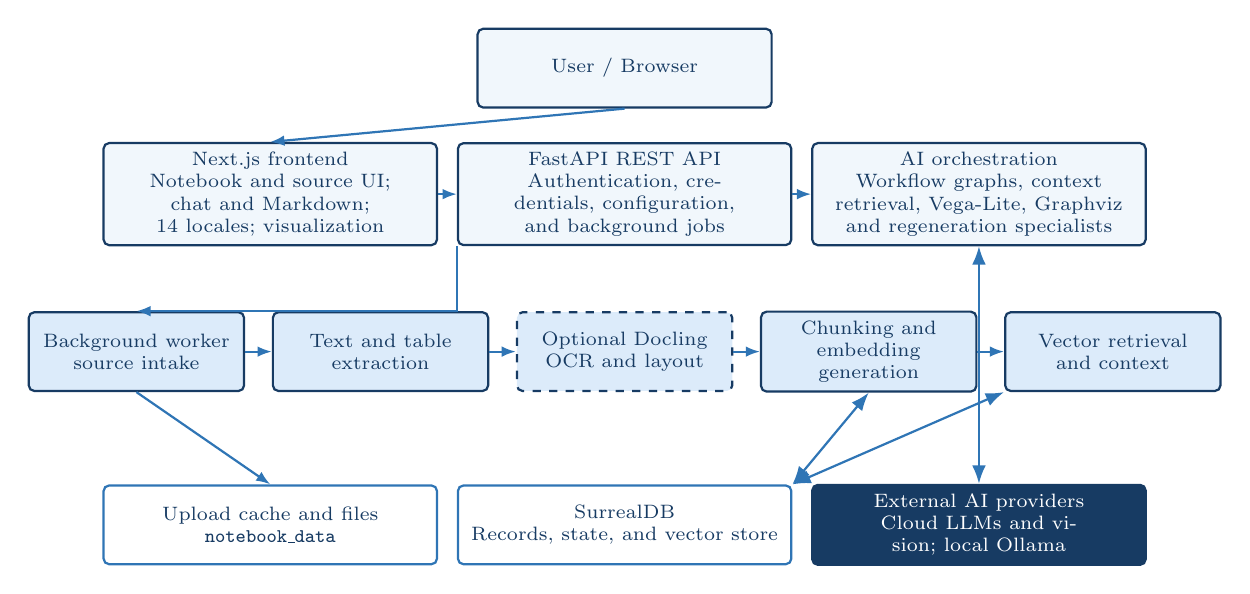
\begin{tikzpicture}[x=1cm,y=1cm,
  component/.style={draw=docintelNavy,fill=docintelPaleBlue,text=docintelNavy,rounded corners=2pt,align=center,font=\scriptsize,line width=0.8pt,minimum height=10mm},
  process/.style={component,fill=docintelLightBlue,text width=25mm,minimum width=25mm},
  storage/.style={component,fill=white,draw=docintelBlue,text width=40mm,minimum width=40mm},
  provider/.style={component,fill=docintelNavy,text=white,text width=40mm,minimum width=40mm},
  flow/.style={-{Latex[length=1.8mm]},draw=docintelBlue,line width=0.8pt},
  exchange/.style={<->,>=Latex,draw=docintelBlue,line width=0.8pt}]
\node[component,text width=35mm,minimum width=35mm] (browser) at (0,6.8) {User / Browser};
\node[component,text width=40mm,minimum width=40mm] (frontend) at (-4.5,5.2) {Next.js frontend\\Notebook and source UI; chat and Markdown; 14 locales; visualization};
\node[component,text width=40mm,minimum width=40mm] (api) at (0,5.2) {FastAPI REST API\\Authentication, credentials, configuration, and background jobs};
\node[component,text width=40mm,minimum width=40mm] (orchestration) at (4.5,5.2) {AI orchestration\\Workflow graphs, context retrieval, Vega-Lite, Graphviz and regeneration specialists};
\node[process] (intake) at (-6.2,3.2) {Background worker\\source intake};
\node[process] (extract) at (-3.1,3.2) {Text and table\\extraction};
\node[process,dashed] (ocr) at (0,3.2) {Optional Docling\\OCR and layout};
\node[process] (embed) at (3.1,3.2) {Chunking and\\embedding generation};
\node[process] (context) at (6.2,3.2) {Vector retrieval\\and context};
\node[storage] (uploads) at (-4.5,1.0) {Upload cache and files\\\texttt{notebook\_data}};
\node[storage] (database) at (0,1.0) {SurrealDB\\Records, state, and vector store};
\node[provider] (providers) at (4.5,1.0) {External AI providers\\Cloud LLMs and vision; local Ollama};
\draw[flow] (browser.south) -- (frontend.north);
\draw[flow] (frontend.east) -- (api.west);
\draw[flow] (api.east) -- (orchestration.west);
\draw[flow] (api.south west) |- (intake.north);
\draw[flow] (intake) -- (extract);
\draw[flow] (extract) -- (ocr);
\draw[flow] (ocr) -- (embed);
\draw[flow] (embed) -- (context);
\draw[flow] (intake.south) -- (uploads.north);
\draw[exchange] (embed.south) -- (database.north east);
\draw[exchange] (database.north east) -- (context.south west);
\draw[exchange] (orchestration.south) -- (providers.north);
\end{tikzpicture}%
}
\caption{DocIntel system architecture overview, reconstructed from the supplied architecture document.}
\label{fig:architecture}
\end{figure*}



\begin{figure*}[!t]
\centering
\resizebox{0.92\textwidth}{!}{%
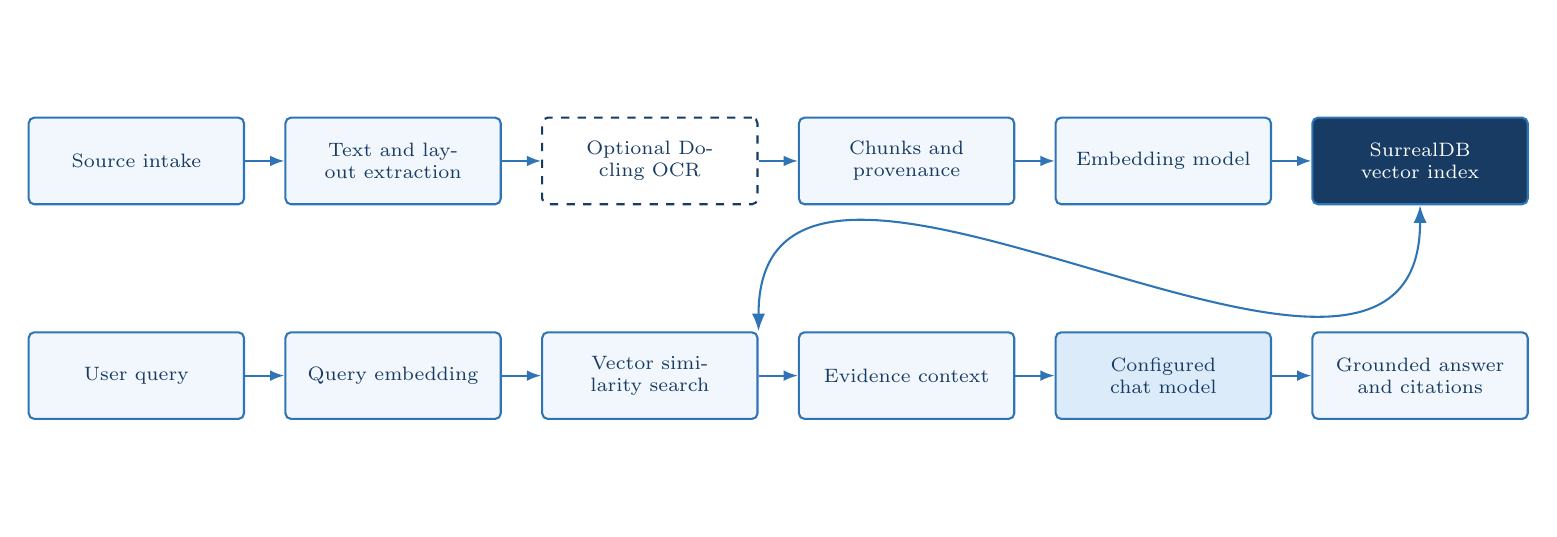
\begin{tikzpicture}[x=1cm,y=1cm,
  stage/.style={draw=docintelBlue,fill=docintelPaleBlue,text=docintelNavy,rounded corners=2pt,align=center,font=\scriptsize,text width=25mm,minimum width=25mm,minimum height=11mm,line width=0.75pt},
  optional/.style={stage,fill=white,dashed,draw=docintelNavy},
  storage/.style={stage,fill=docintelNavy,text=white},
  provider/.style={stage,fill=docintelLightBlue},
  flow/.style={-{Latex[length=1.8mm]},draw=docintelBlue,line width=0.75pt},
  exchange/.style={<->,>=Latex,draw=docintelBlue,line width=0.75pt}]
\node[stage] (source) at (0,3.0) {Source intake};
\node[stage,right=5mm of source] (extract) {Text and layout extraction};
\node[optional,right=5mm of extract] (ocr) {Optional Docling OCR};
\node[stage,right=5mm of ocr] (chunks) {Chunks and provenance};
\node[stage,right=5mm of chunks] (embed) {Embedding model};
\node[storage,right=5mm of embed] (index) {SurrealDB vector index};
\node[stage,below=16mm of source] (query) {User query};
\node[stage,right=5mm of query] (queryembed) {Query embedding};
\node[stage,right=5mm of queryembed] (search) {Vector similarity search};
\node[stage,right=5mm of search] (evidence) {Evidence context};
\node[provider,right=5mm of evidence] (chat) {Configured chat model};
\node[stage,right=5mm of chat] (answer) {Grounded answer and citations};
\draw[flow] (source) -- (extract);
\draw[flow] (extract) -- (ocr);
\draw[flow] (ocr) -- (chunks);
\draw[flow] (chunks) -- (embed);
\draw[flow] (embed) -- (index);
\draw[flow] (query) -- (queryembed);
\draw[flow] (queryembed) -- (search);
\draw[flow] (search) -- (evidence);
\draw[flow] (evidence) -- (chat);
\draw[flow] (chat) -- (answer);
\draw[exchange] (index.south) to[out=-90,in=90,looseness=1.15] (search.north east);
\end{tikzpicture}%
}
\caption{Source indexing and query-time retrieval flow. The vector index stores chunk embeddings and provenance metadata.}
\label{fig:retrieval-dataflow}
\end{figure*}


\subsection{Frontend}
The Next.js frontend provides notebooks, sources, settings, search, chat, Markdown, podcast controls, and visualization rendering. The interface uses browser-language detection, a saved preference, and an English fallback. Selecting an interface locale does not itself translate source text; translation or multilingual understanding depends on a configured language or embedding model when appropriate \cite{docintel}.

\subsection{API and Background Processing}
FastAPI is responsible for authentication, provider credentials, model configuration, source creation, notebook operations, chat, transformations, search, jobs, and visualization endpoints. Long-running extraction, embedding generation, transformation, and podcast jobs are delegated through a worker/runtime path so that requests can be processed asynchronously. Processing status should be checked through the API or user interface rather than assumed complete after upload \cite{docintel}.

\subsection{AI Orchestration}
LangGraph/LangChain-oriented workflows assemble prompts and source context, invoke a configured provider, and stream output. Chat and embeddings can be configured independently. This separation permits a local embedding model with a cloud language model, or both remote, local, or mixed according to latency, cost, and privacy requirements \cite{langgraph,docintel}.

\subsection{Framework and Module Responsibilities}
The implemented modules have distinct responsibilities and expose provider-specific components through stable application boundaries:
\begin{itemize}
 \item \textbf{Source-intake module:} normalizes uploaded files, URLs, text, images, and media into source records and stores integrity metadata.
 \item \textbf{Extraction module:} uses format-specific handlers and an optional Docling runtime for layout-aware text, OCR, table, and document structure extraction.
 \item \textbf{Chunking and metadata module:} divides extracted content while retaining source, document, page, position, and processing information needed for citations.
 \item \textbf{Embedding module:} converts chunks into vectors using a provider-selected embedding model and updates SurrealDB records.
 \item \textbf{Retrieval module:} embeds queries in the compatible vector space, selects relevant chunks, and constructs bounded evidence context.
 \item \textbf{Orchestration module:} implemented with LangGraph/LangChain concepts, manages strategy, partial answers, synthesis, tool prompts, conversation state, and provider invocation.
 \item \textbf{Generation module:} produces notebook chat, source chat, summaries, transformations, and final answers through provider-selectable chat models.
 \item \textbf{Visualization module:} renders Vega-Lite charts, Graphviz DOT diagrams, explicit Mermaid regeneration, optional SVG/Python plots, format labels, regeneration menus, and sanitized downloadable artifacts.
 \item \textbf{Storage and deployment modules:} SurrealDB and Docker volumes persist records and files, while Docker Compose defines the application runtime.
 \item \textbf{Security and configuration modules:} encrypt credentials, enforce configured application access, isolate runtime data, and sanitize external-facing output.
\end{itemize}

\subsection{Storage and Persistence}
SurrealDB stores notebooks, sources, notes, processing state, credential metadata, jobs, and vector records. Uploaded source files and caches are under \texttt{notebook\_data}; database state is under \texttt{surreal\_data}. These volume semantics are important for backup, migration, and data-retention policy \cite{docintel,surrealdb}.

\section{Document Processing Pipeline}
\begin{figure*}[!t]
\centering
\resizebox{0.84\textwidth}{!}{%
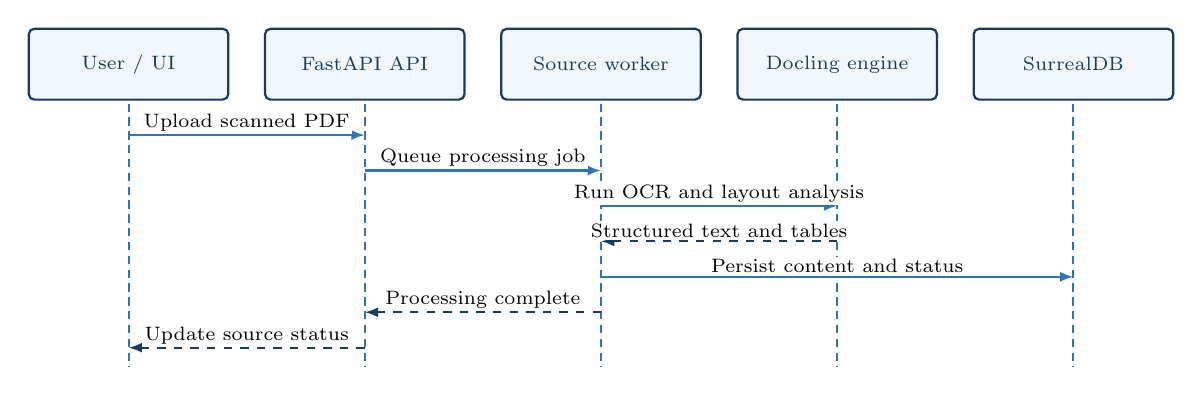
\begin{tikzpicture}[x=1cm,y=1cm,
  participant/.style={draw=docintelNavy,fill=docintelPaleBlue,text=docintelNavy,rounded corners=2pt,align=center,font=\scriptsize,text width=23mm,minimum width=23mm,minimum height=9mm,line width=0.8pt},
  lifeline/.style={draw=docintelBlue,densely dashed,line width=0.7pt},
  request/.style={-{Latex[length=1.7mm]},draw=docintelBlue,line width=0.8pt},
  response/.style={-{Latex[length=1.7mm]},draw=docintelNavy,dashed,line width=0.8pt}]
\node[participant] (ui) at (0,3.5) {User / UI};
\node[participant] (api) at (3,3.5) {FastAPI API};
\node[participant] (worker) at (6,3.5) {Source worker};
\node[participant] (docling) at (9,3.5) {Docling engine};
\node[participant] (db) at (12,3.5) {SurrealDB};
\foreach \x in {0,3,6,9,12} {\draw[lifeline] (\x,3.0) -- (\x,-0.35);}
\draw[request] (0,2.6) -- node[above,font=\scriptsize,fill=white,inner sep=1pt] {Upload scanned PDF} (3,2.6);
\draw[request] (3,2.15) -- node[above,font=\scriptsize,fill=white,inner sep=1pt] {Queue processing job} (6,2.15);
\draw[request] (6,1.7) -- node[above,font=\scriptsize,fill=white,inner sep=1pt] {Run OCR and layout analysis} (9,1.7);
\draw[response] (9,1.25) -- node[above,font=\scriptsize,fill=white,inner sep=1pt] {Structured text and tables} (6,1.25);
\draw[request] (6,0.8) -- node[above,font=\scriptsize,fill=white,inner sep=1pt] {Persist content and status} (12,0.8);
\draw[response] (6,0.35) -- node[above,font=\scriptsize,fill=white,inner sep=1pt] {Processing complete} (3,0.35);
\draw[response] (3,-0.1) -- node[above,font=\scriptsize,fill=white,inner sep=1pt] {Update source status} (0,-0.1);
\end{tikzpicture}%
}
\caption{OCR and extraction sequence for a scanned source, reconstructed from the supplied architecture document.}
\label{fig:ocr-sequence}
\end{figure*}


\subsection{Source Ingestion}
Supported sources are normalized into application content and metadata. Files include text-bearing formats such as PDF, DOCX, and XLSX, while URLs, text, audio, and video use their respective content handlers. Format-specific extraction should preserve source identifiers so that responses can refer to original source records and retrieved evidence \cite{docintel}.

\subsection{Extraction and OCR}
DocIntel uses content-core extraction as the baseline and may enable Docling as an optional runtime. When enabled, Docling can perform layout-aware processing, OCR, table extraction, formula recognition, reading-order analysis, and image-oriented processing. OCR must be evaluated separately from native-text extraction: a text-native PDF may bypass OCR regardless of image quality, and extraction settings can change the output \cite{docling2024,doclingDocs2026}.

\subsection{Retrieval and Generation}
Extracted text is segmented into chunks and associated with source metadata. The embedding provider generates vector representations stored by the application. A retrieval request searches for relevant vectors and metadata, assembles context, and invokes a selected language model. The model may also rely on notebook instructions, source instructions, conversation state, and transformation prompts \cite{docintel}.

The conceptual workflow is
\begin{equation}
 R(q)=\operatorname{TopK}_{c \in C}\left(\cos(E_q(q),E_c(c))\right),
\end{equation}
where $q$ is the query, $C$ is the source corpus, $E_q$ and $E_c$ are embedding functions, and the top-$K$ contexts are passed to generation. If the embedding model changes, vectors from different models should not be mixed. Existing sources generally require re-embedding for retrieval consistency.

\section{Visual Explanation and Multimodal Features}
DocIntel uses Matplotlib/Python for default data charts and Graphviz DOT for relationships and architecture diagrams. Vega-Lite JSON and Mermaid remain available as explicit formats through regeneration. Rendered cards identify their format and support PNG/SVG downloads and source copying; Mermaid and SVG output use strict rendering and sanitization. Python plotting applies abstract-syntax-tree validation, restricted imports, private-attribute restrictions, timeouts, output limits, temporary working directories, and process controls. These controls reduce risk but do not constitute an untrusted-code sandbox suitable for public tenants \cite{docintel}.

The visualization capability should be considered generated presentation logic rather than ground-truth analysis. Numerical claims should be calculated reproducibly and checked against source evidence.

\section{Provider Configuration}
DocIntel supports provider credentials for cloud and local systems, including OpenAI-compatible providers and Ollama. The provider registry determines required credentials and supported modalities. Model categories include language/chat, embedding, speech-to-text, and text-to-speech. Chat models must not be treated as embedding models unless the provider explicitly supports an embedding modality \cite{docintel,ollama}.

Google Gemini Embedding 001 is an embedding option when the Google provider credential is configured. Newer or multimodal embedding models should be used only after confirming compatibility with the installed DocIntel/provider contract. Embedding dimensions and provider compatibility affect model migration; changing embeddings requires re-processing existing sources \cite{googleembed}.

As an offline option, Ollama can host models such as \texttt{nomic-embed-text}. For Docker deployment, the host may need to be addressed as \texttt{host.docker.internal}; this differs between operating systems and firewall configurations \cite{ollama}.

\section{Deployment Methodology}
DocIntel uses a persistent Docker deployment. A typical setup is:
\begin{lstlisting}[language=bash,caption={Deployment commands},float=tb]
cp .env.example .env
openssl rand -hex 32
# Configure OPEN_NOTEBOOK_ENCRYPTION_KEY in .env
docker compose up -d --build
docker compose ps
docker compose logs -f open_notebook
\end{lstlisting}

The default user-facing ports are 8502 for the Next.js interface and 5055 for the API. SurrealDB is bound locally in the documented deployment. Stable encryption keys are required: replacing the key can make existing encrypted credentials unreadable. Provider credentials should be configured through the UI and not committed to version control \cite{docintel}.

\section{Security and Privacy}
DocIntel exposes several important privacy boundaries. Provider credentials are encrypted with a configured application key. Application files and runtime state persist separately from SurrealDB. Public repositories should exclude \texttt{.env}, uploads, databases, API keys, notebooks, caches, and generated runtime state. Cloud providers receive source context when their model is selected and queried \cite{docintel}.

Additional controls include strict Mermaid rendering, SVG sanitization, restricted Python execution, host/port isolation, and configurable authentication or password protection. A public deployment should also add HTTPS, authenticated administrative routes, database access controls, source-size limits, rate limiting, audit logging, backup policies, and isolated execution for untrusted visualizations. These recommendations do not imply that every control is currently implemented.

\section{Evaluation}
\subsection{Implementation Validation}
The repository has separate backend visualization tests and frontend test suites. The development snapshot reported during project work included seven backend visualization tests and 182 frontend tests across 35 files. The frontend production build and Docker Compose configuration were also reported as validated. These are author-reported snapshots, not independently reproduced results, and should be regenerated with the software version used for publication \cite{docintel}.

\subsection{Corpus and Benchmark}
The final comparison used 14 railway-domain documents consisting of 8 PDF, 3 DOCX, and 3 XLSX files. All source files, extracted-text files, counts, paths, and SHA-256 hashes were retained in the evaluation corpus. Automated extraction succeeded for all 14 documents, after which 10 fixed source-grounded questions were prepared across numeric facts, table lookups, technical specifications, threshold values, incidents, and spreadsheet aggregations.

Direct-model runs supplied the complete extracted text of each relevant document and returned final answers through OpenCode CLI JSON event logs. DocIntel was invoked through its source-grounded search API and used Gemini 3.5 Flash Lite for query strategy, partial answer generation, and final synthesis. This comparison is system-level rather than a matched isolated-generation test: direct models received full extracted text, whereas DocIntel additionally performed ingestion, chunking, embedding, retrieval, synthesis, and citation assembly.

\begin{table}[!t]
\centering
\caption{Extraction validation for the 14-document railway corpus}
\label{tab:extract}
\small
\begin{tabular}{lccc}
\toprule
\rowcolor{docintelLightBlue}
Format & Files & Successful & Result \\
\midrule
PDF & 8 & 8 & Native text/layout \\
DOCX & 3 & 3 & Paragraphs extracted \\
XLSX & 3 & 3 & Worksheet rows/cells processed \\
\midrule
Total & 14 & 14 & 100\% successful \\
\bottomrule
\end{tabular}
\end{table}

\subsection{Question Answering Results}
Human semantic grading was applied to usable answers. The comparison uses both coverage accuracy and conditional correctness. Coverage is the number of correct answers divided by all 10 questions; conditional correctness is the number of correct answers divided by usable textual responses. Provider failures, incomplete JSON-event output, CLI exit anomalies, and semantic incorrectness are not conflated.

\begin{table*}[!t]
\centering
\caption{DocIntel and direct-model source-grounded comparison}
\label{tab:model-results}
\small
\setlength{\tabcolsep}{4pt}
\begin{tabular}{lccccc}
\toprule
\rowcolor{docintelLightBlue}
System/model & Correct / 10 & Usable text & Coverage & Conditional correctness & Mean latency (s) \\
\midrule
DocIntel + Gemini 3.5 Flash Lite & 10 & 10 & 100\% & 100\% & 14.11 \\
Thinking Machines Inkling Small Free & 10 & 10 & 100\% & 100\% & 2.80 \\
Cohere North Mini Code Free & 8 & 8 & 80\% & 100\% & 2.99 \\
GLM 5.3 Flash Free & 2 & 2 & 20\% & 100\% & 3.12 \\
Nemotron 3.5 Lightning Free & 2 & 2 & 20\% & 100\% & 8.92 \\
Nemotron 3.5 Super VL Free & 2 & 2 & 20\% & 100\% & 26.15 \\
\bottomrule
\end{tabular}
\end{table*}


\begin{figure*}[!t]
\centering
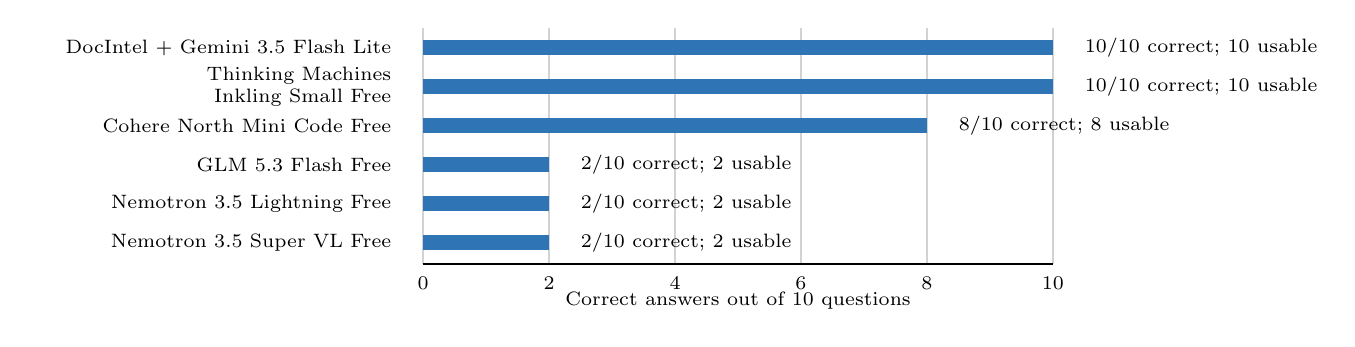
\begin{tikzpicture}[x=0.8cm,y=0.55cm]
\foreach \x in {0,2,4,6,8,10} {
  \draw[gray!35] (\x,0.7) -- (\x,6.15);
  \node[font=\scriptsize,below] at (\x,0.62) {\x};
}
\draw[black,line width=0.7pt] (0,0.7) -- (10,0.7);
\node[anchor=east,align=right,text width=45mm,font=\scriptsize] at (-0.35,5.7) {DocIntel + Gemini 3.5 Flash Lite};
\fill[docintelBlue] (0,5.53) rectangle (10,5.87);
\node[anchor=west,font=\scriptsize] at (10.35,5.7) {10/10 correct; 10 usable};
\node[anchor=east,align=right,text width=45mm,font=\scriptsize] at (-0.35,4.8) {Thinking Machines Inkling Small Free};
\fill[docintelBlue] (0,4.63) rectangle (10,4.97);
\node[anchor=west,font=\scriptsize] at (10.35,4.8) {10/10 correct; 10 usable};
\node[anchor=east,align=right,text width=45mm,font=\scriptsize] at (-0.35,3.9) {Cohere North Mini Code Free};
\fill[docintelBlue] (0,3.73) rectangle (8,4.07);
\node[anchor=west,font=\scriptsize] at (8.35,3.9) {8/10 correct; 8 usable};
\node[anchor=east,align=right,text width=45mm,font=\scriptsize] at (-0.35,3.0) {GLM 5.3 Flash Free};
\fill[docintelBlue] (0,2.83) rectangle (2,3.17);
\node[anchor=west,font=\scriptsize] at (2.35,3.0) {2/10 correct; 2 usable};
\node[anchor=east,align=right,text width=45mm,font=\scriptsize] at (-0.35,2.1) {Nemotron 3.5 Lightning Free};
\fill[docintelBlue] (0,1.93) rectangle (2,2.27);
\node[anchor=west,font=\scriptsize] at (2.35,2.1) {2/10 correct; 2 usable};
\node[anchor=east,align=right,text width=45mm,font=\scriptsize] at (-0.35,1.2) {Nemotron 3.5 Super VL Free};
\fill[docintelBlue] (0,1.03) rectangle (2,1.37);
\node[anchor=west,font=\scriptsize] at (2.35,1.2) {2/10 correct; 2 usable};
\node[font=\scriptsize] at (5,-0.15) {Correct answers out of 10 questions};
\end{tikzpicture}
\caption{Question coverage by system in the fixed benchmark. Lower counts for several direct models coincide with provider or process failures and do not measure standalone model quality.}
\label{fig:qa-coverage}
\end{figure*}

In the final DocIntel run, q04 and q05 were verified again after provider-sensitive retries and all 10 answers were correct. Inkling produced usable text for every question and was correct on every response. Cohere returned 8 usable answers and correctly answered all of them, but q09 and q10 produced provider/session failures. GLM, Nemotron Lightning, and Nemotron Super VL returned complete usable answer text only for q01 and q02 in the reported run. The remaining invocations produced incomplete CLI JSON event records or session failures, so their 20\% coverage does not establish 20\% model intelligence and must not be interpreted as a broad quality ranking. No response-quality difference should be inferred from the exact number of provider failures alone without rerunning the complete benchmark and recording process exit conditions.

The 26.15-second Super VL mean includes two textual runs, including one invocation that returned a correct answer despite a non-zero process exit. The supplied benchmark used extracted text rather than page images. Consequently, Super VL's vision capability was not exercised and this experiment does not compare vision OCR or chart interpretation.

\subsection{Metrics and Evaluation Dimensions}
Semantic correctness answers whether a response is equivalent to the verified fact, while coverage answers whether a complete end-to-end invocation produced an accepted response. A publication-quality evaluation should additionally record retrieval Recall@$K$, MRR, NDCG, citation precision and recall, answer faithfulness, unsupported claims, latency, provider cost, repeated-run variance, and human preference. Vision evaluation requires CER, WER, layout-tree similarity, table-cell accuracy, formula recognition, chart-data extraction, and grounded visual question answering \cite{omnidocbench2025,ocrBenchV2,ragEval2024}. The reported benchmark does not establish these dimensions.

\subsection{Recommended OCR Evaluation}
Because OCR accuracy cannot be inferred from native-format extraction, publication-grade evaluation should use a corpus with known ground truth. Suggested metrics include character error rate (CER), word error rate (WER), table-cell accuracy, reading-order similarity, and formula-recognition accuracy \cite{omnidocbench2025,ocrBenchV2}. Evaluation should report per-language and per-document-type results and include:
\begin{itemize}
 \item low-resolution scans;
 \item skew and rotation;
 \item shadows and uneven illumination;
 \item multi-column pages;
 \item handwritten and mixed-language text;
 \item embedded tables, formulas, captions, and stamps; and
 \item native PDF, scanned PDF, and image comparisons.
\end{itemize}

\subsection{Recommended Retrieval Evaluation}
A reusable retrieval benchmark should contain verified questions, source citations, and expected passages. Recommended metrics are Recall@$K$, Mean Reciprocal Rank, NDCG, answer faithfulness, citation support, and human preference \cite{ragEval2024}. Experiments should compare at least:
\begin{enumerate}
 \item native extraction with no OCR;
 \item Docling/OCR-enabled extraction;
 \item Google Gemini Embedding 001;
 \item a local Ollama embedding model; and
 \item multiple chunk sizes and top-$K$ retrieval depths.
\end{enumerate}

\section{Reproducibility and Experimental Protocol}
\begin{enumerate}
 \item Start from a clean commit and record its hash, image identifiers, dependency lockfiles, and Docling version.
 \item Configure a stable encryption key and keep provider credentials outside version control.
 \item Import a fixed corpus and retain its checksums.
 \item Record extraction-engine, OCR, chunking, embedding, language-model, temperature, and retrieval settings.
 \item Run source processing and wait for completion status.
 \item Export extracted text and metadata without exposing private source content.
 \item Execute retrieval and answer-generation queries using a fixed seed when supported.
 \item Record provider, latency, cost, token usage, and generated answer.
 \item Compare only runs that use compatible embedding spaces.
 \item Rebuild embeddings after changing embedding providers or models.
 \item Perform human verification for provenance and factual faithfulness.
 \item Publish commands, configuration templates, aggregate metrics, failed cases, and environment limitations.
\end{enumerate}

A reproducible result must distinguish software compatibility from model quality. Container health, successful processing, and API connectivity do not establish answer correctness.

\section{Threats to Validity}
\begin{itemize}
 \item \textbf{Corpus bias:} The existing railway corpus is small and synthetic.
 \item \textbf{OCR bias:} Native-format extraction does not measure OCR.
 \item \textbf{Provider drift:} Cloud model behavior, prices, quotas, and identifiers can change.
 \item \textbf{Embedding non-comparability:} Vectors from different models cannot be compared directly.
 \item \textbf{Metric instability:} Automatically generated answers require citation and faithfulness verification.
 \item \textbf{Prompt sensitivity:} Retrieval and generation can vary with instructions and temperature.
 \item \textbf{Privacy leaks:} Shared prompts may transmit source text to configured cloud providers.
 \item \textbf{Localization coverage:} Interface translation is not equivalent to faithful multilingual content understanding.
\end{itemize}

\section{Limitations and Future Work}
Future work should include larger multi-domain OCR benchmarks; systematic table and formula datasets; citation-level evidence evaluation; adversarial source tests; provenance visualization; incremental and differential embedding; privacy-preserving local inference; user studies; and stronger tenant isolation for public deployments. Benchmarks should include OCR engines such as Tesseract, PaddleOCR, and Docling under controlled hardware and model configurations.

Additional engineering work includes immutable document snapshots, chunk provenance, field-level confidence, source-change auditing, encrypted backup procedures, and objective evaluation of response latency and token cost. The Python plotting environment should be moved to a stronger isolated service before accepting untrusted third-party code.

\balance
\section{Conclusion}
DocIntel presents an integrated architecture for private document research. It combines heterogeneous ingestion, optional layout-aware OCR, configurable embeddings, retrieval, provider-flexible generation, notebooks, multilingual interface support, and downloadable visual explanations. Its architecture is designed to avoid vendor lock-in while keeping storage and credentials under application control.

The final comparison confirms extraction for all 14 documents in the railway corpus. In a fixed 10-question source-grounded benchmark, DocIntel reached 10/10 semantic correctness, and the direct Inkling Small baseline also reached 10/10; Inkling had lower measured direct-response latency, while Cohere answered all 8 usable responses correctly but failed two provider invocations. Partial model coverage in GLM, Nemotron Lightning, and Nemotron Super VL prevents meaningful quality ranking and should be investigated through provider-session reruns. These results are limited by the small corpus, one question set, one application run, and incomplete repeated-run statistics.

Accordingly, the paper supports provider-flexible system integration and correctness for the measured benchmark, but it does not claim OCR, vision, retrieval ranking, or statistical generalization performance. Future publication should freeze retrieval settings, include independently verified passages and multiple human graders, report repeated runs and confidence intervals, compare text and rendered-page baselines fairly, and expand the corpus across domains and document layouts.

\appendices
\section{Configuration Template}
\begin{lstlisting}[caption={Illustrative environment template}]
OPEN_NOTEBOOK_ENCRYPTION_KEY=<generate-a-stable-random-key>
OPEN_NOTEBOOK_ENABLE_DOCLING=true
SURREAL_USER=root
SURREAL_PASSWORD=<choose-a-private-password>
SURREAL_NAMESPACE=open_notebook
SURREAL_DATABASE=open_notebook
\end{lstlisting}

\section{Data and Software Availability}
The project source repository and execution instructions should be published with dependency lockfiles and Docker Compose configuration. API keys, private documents, databases, notebooks, and runtime data must not be included. Synthetic documents may be distributed if cleared for redistribution; private or unpublished source data should be excluded. A reproducible release should identify the software commit, container image digest, Docling version, provider/model identifiers, and test commands.

\begin{thebibliography}{13}
\bibitem{ragSurvey2024}
S. Gupta, R. Ranjan, and S. N. Singh, ``A Comprehensive Survey of Retrieval-Augmented Generation (RAG): Evolution, Current Landscape and Future Directions,'' arXiv:2410.12837, 2024. [Online]. Available: \url{https://arxiv.org/abs/2410.12837}

\bibitem{docintel}
S. Mittal, ``DocIntel: Document Intelligence Workspace,'' GitHub repository. [Online]. Available: \url{https://github.com/Samar23dev/DocIntel}. Accessed: Oct. 31, 2026.

\bibitem{tesseract2026}
Tesseract OCR Contributors, ``Tesseract OCR Engine,'' ver. 5.5.4, Oct. 2026. [Online]. Available: \url{https://github.com/tesseract-ocr/tesseract/releases/tag/5.5.4}

\bibitem{docling2024}
C. Auer, M. Lysak, A. Nassar, et al., ``Docling Technical Report,'' arXiv:2408.09869, 2024. [Online]. Available: \url{https://arxiv.org/abs/2408.09869}

\bibitem{doclingDocs2026}
Docling Contributors, ``Docling Documentation.'' [Online]. Available: \url{https://github.com/docling-project/docling}. Accessed: Oct. 31, 2026.

\bibitem{omnidocbench2025}
L. Ouyang, Y. Qu, H. Zhou, et al., ``OmniDocBench: Benchmarking Diverse PDF Document Parsing with Comprehensive Annotations,'' in \emph{Proceedings of the IEEE/CVF Conference on Computer Vision and Pattern Recognition}, 2025, pp. 24838--24848.

\bibitem{ocrBenchV2}
L. Fu, Z. Kuang, J. Song, et al., ``OCRBench v2: An Improved Benchmark for Evaluating Large Multimodal Models on Visual Text Localization and Reasoning,'' in \emph{Advances in Neural Information Processing Systems}, vol. 38, Datasets and Benchmarks Track, 2025, doi: 10.52202/085713-3253.

\bibitem{paddleocr}
PaddleOCR Contributors, ``PaddleOCR: Multilingual OCR Toolkit,'' GitHub repository. [Online]. Available: \url{https://github.com/PaddlePaddle/PaddleOCR}. Accessed: Oct. 31, 2026.

\bibitem{surrealdb}
SurrealDB, ``SurrealDB Documentation.'' [Online]. Available: \url{https://surrealdb.com/docs}. Accessed: Oct. 31, 2026.

\bibitem{langgraph}
LangChain, ``LangGraph Documentation.'' [Online]. Available: \url{https://docs.langchain.com/oss/python/langgraph/overview}. Accessed: Oct. 31, 2026.

\bibitem{ollama}
Ollama, ``Ollama Documentation.'' [Online]. Available: \url{https://docs.ollama.com/}. Accessed: Oct. 31, 2026.

\bibitem{googleembed}
Google, ``Gemini Embeddings Documentation.'' [Online]. Available: \url{https://ai.google.dev/gemini-api/docs/embeddings}. Accessed: Oct. 31, 2026.

\bibitem{ragEval2024}
H. Yu, A. Gan, K. Zhang, S. Tong, Q. Liu, and Z. Liu, ``Evaluation of Retrieval-Augmented Generation: A Survey,'' arXiv:2405.07437, 2024. [Online]. Available: \url{https://arxiv.org/abs/2405.07437}
\end{thebibliography}


\end{document}
